\chapter{Implementacja prototypu systemu}
\label{cha:ImplementacjaPrototypu}

\section{Co zostało zaimplementowane}

Prototyp systemu dostępny jest on-line pod adresem \url{http://facewithme.com}. Przy tworzeniu prototypu systemu skupiono się na 4 elementach systemu (szczegóły architektury znajdują się \namedref{sec:EtapIwstepnaArchitekturaSystemu}):

\begin{packed_item}
    \item{Interfejs WWW}
    \item{baza danych}
    \item{serwer RTMFP}
    \item{Mobile Broadcaster}
    \item{Browser Receiver}
\end{packed_item}

Dzięki wybraniu ww. elementów udało się stworzyć system zdolny do przetestowania transmisji wideo pomiędzy Mobile Broadcaster, a Browser Receiver, za pomocą technologii Adobe P2P Multicast. Interfejs WWW umożliwia dodatkowo ładną prezentację oraz wyszukiwanie stream'ów w zadanej lokalizacji czy też personalizację ustawień. Niżej przedstawiono listę elementów systemu wraz z funkcjami jakie udało się zaimplementować.

\newpage
\textbf{Interfejs WWW}
\begin{packed_item}
    \item{system rejestracji użytkownika (\url{http://facewithme.com/accounts/register})
        \begin{center}
            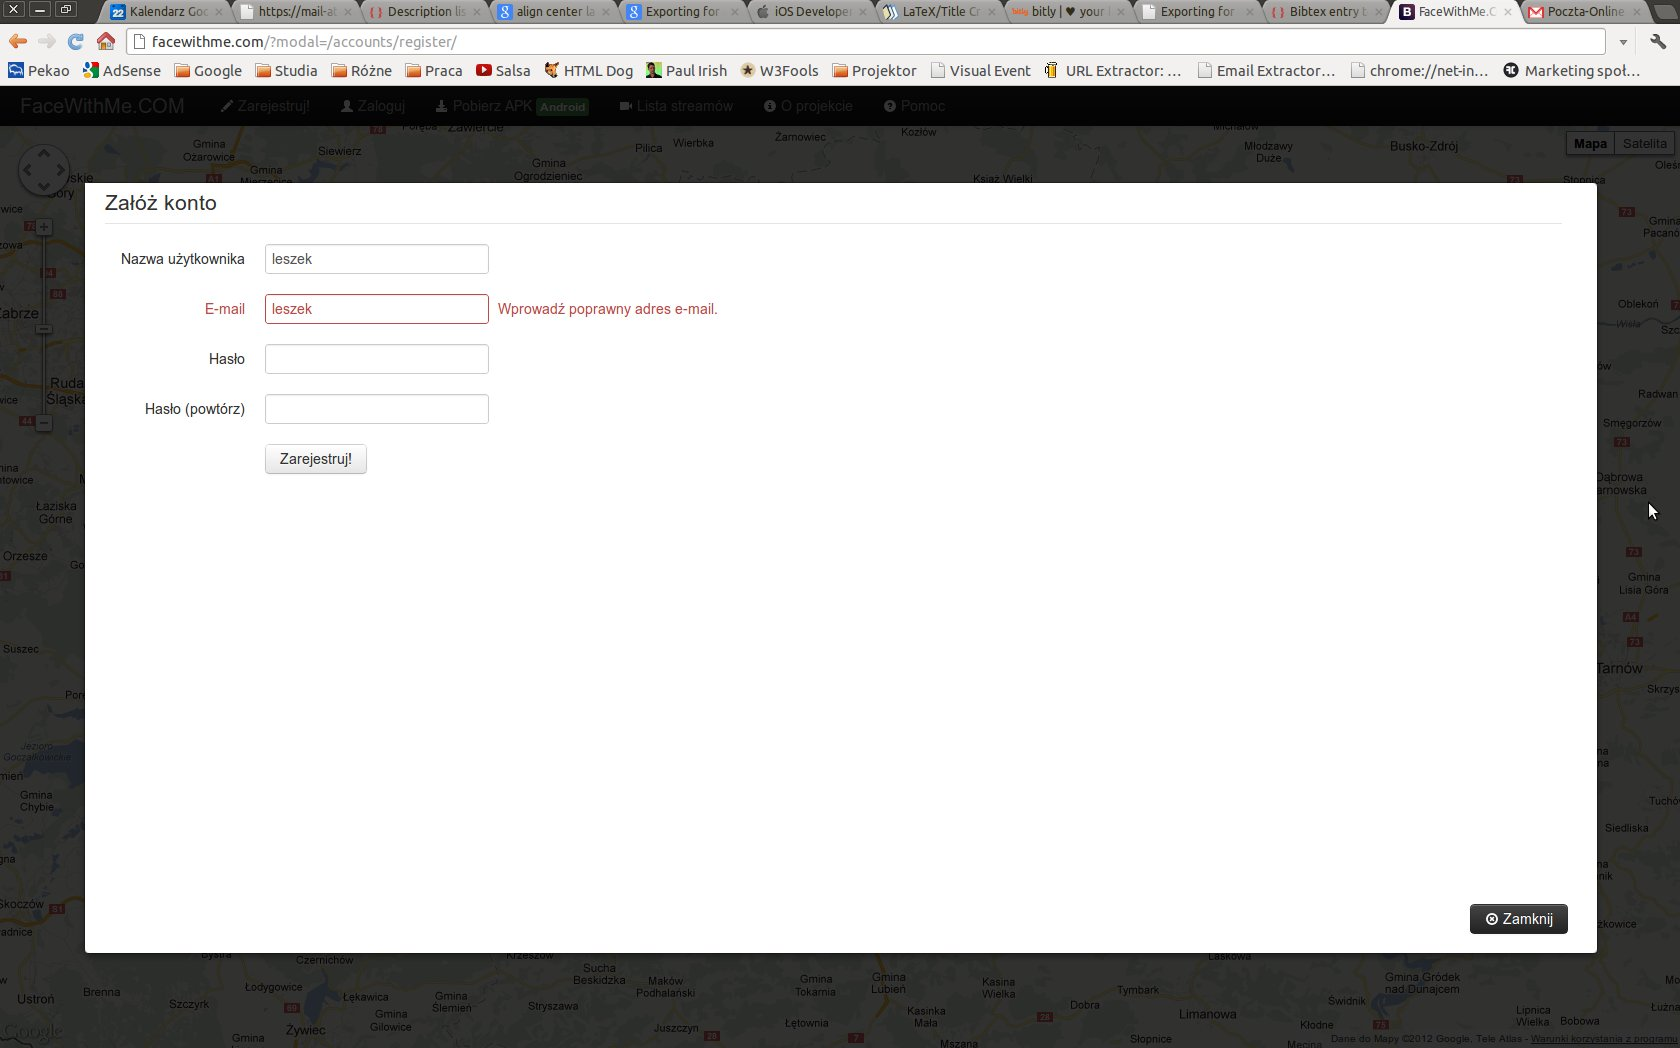
\includegraphics[width=\textwidth]{img/screens/interfejs_www/rejestracja.jpg}
        \end{center}
    }
    \item{system logowania użytkownika (\url{http://facewithme.com/accounts/login})
        \begin{center}
            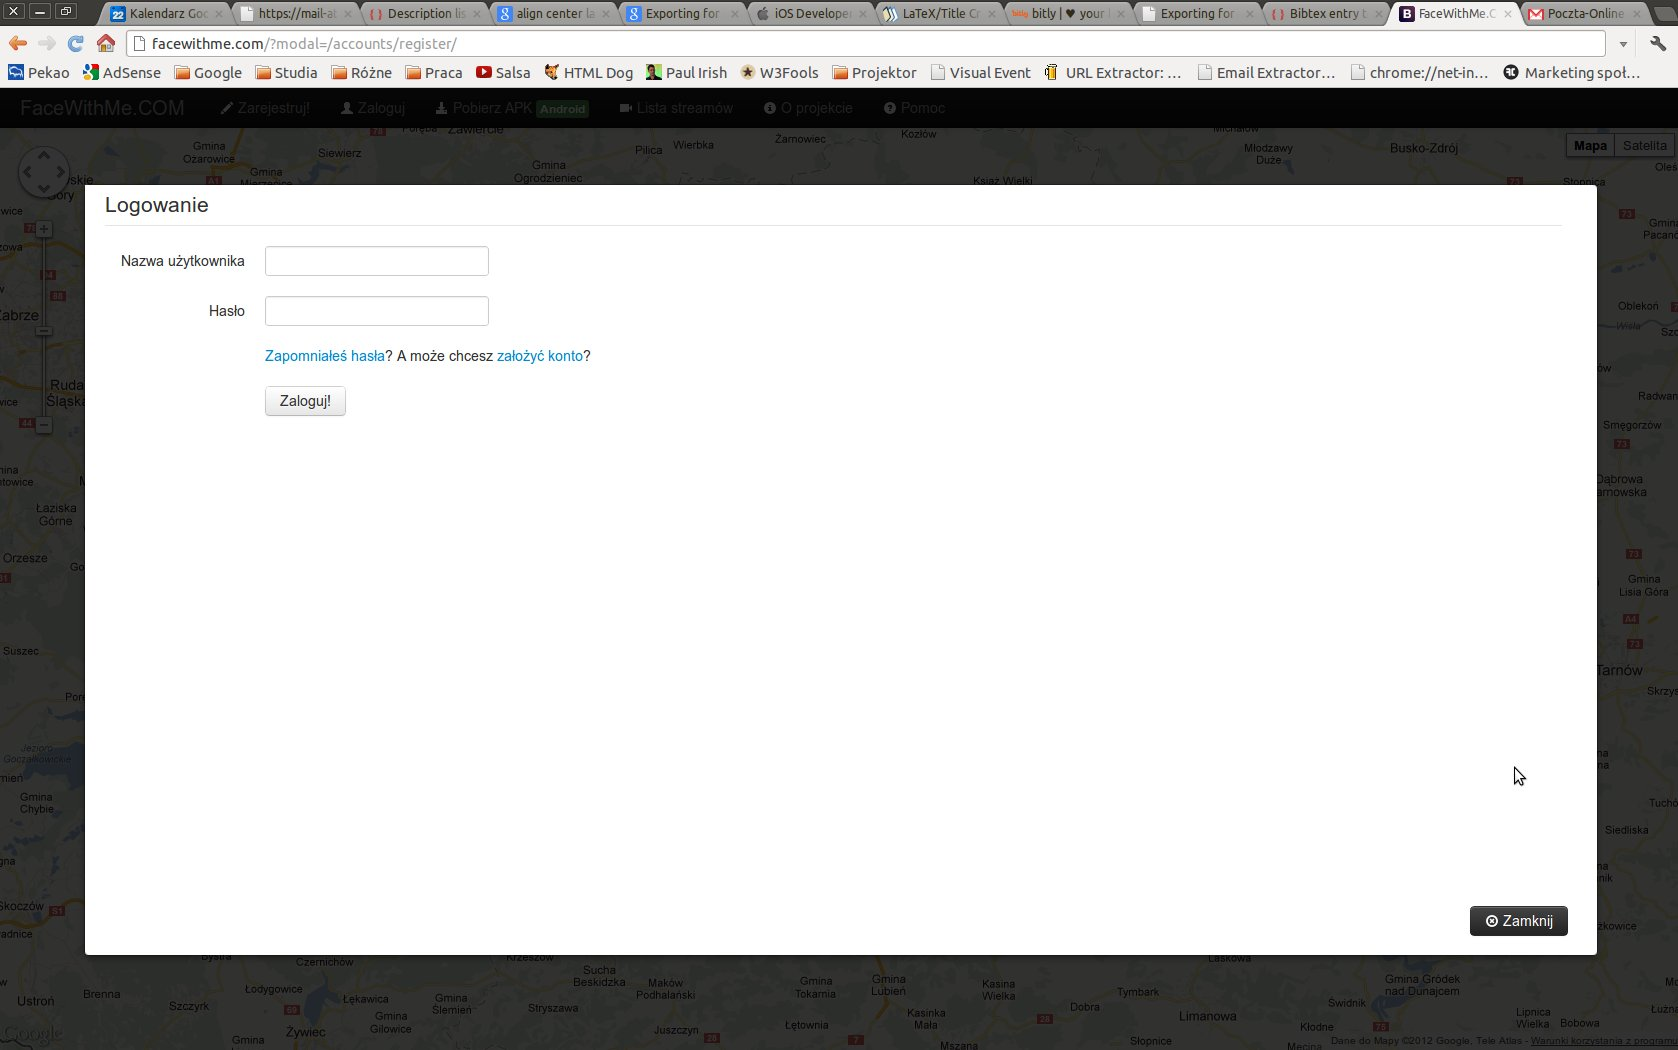
\includegraphics[width=\textwidth]{img/screens/interfejs_www/logowanie.jpg}
        \end{center}
    }
    \item{panel administracyjny do zarządzania stream'ami, kategoriami i użytkownikami (\url{http://facewithme.com/admin})
        \begin{center}
            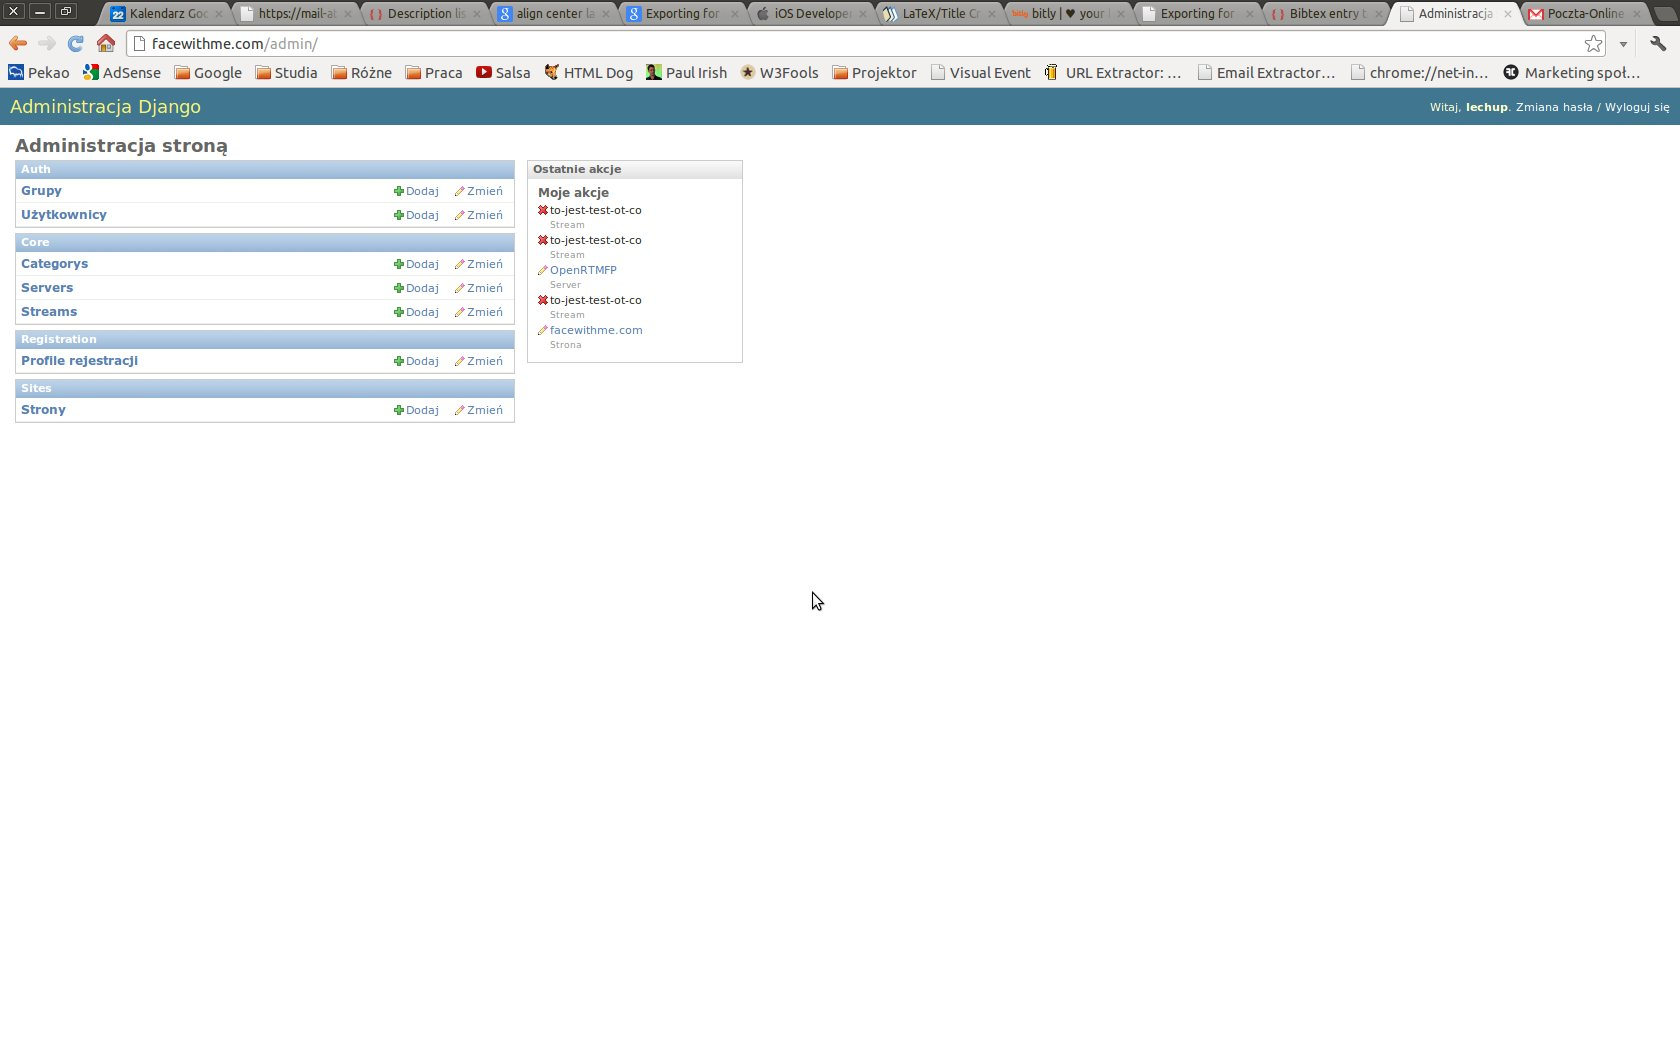
\includegraphics[width=\textwidth]{img/screens/interfejs_www/panel-administracyjny.jpg}
        \end{center}
    }
    \item{interaktywną mapę prezentującą stream'y (\url{http://facewithme.com})
        \begin{center}
            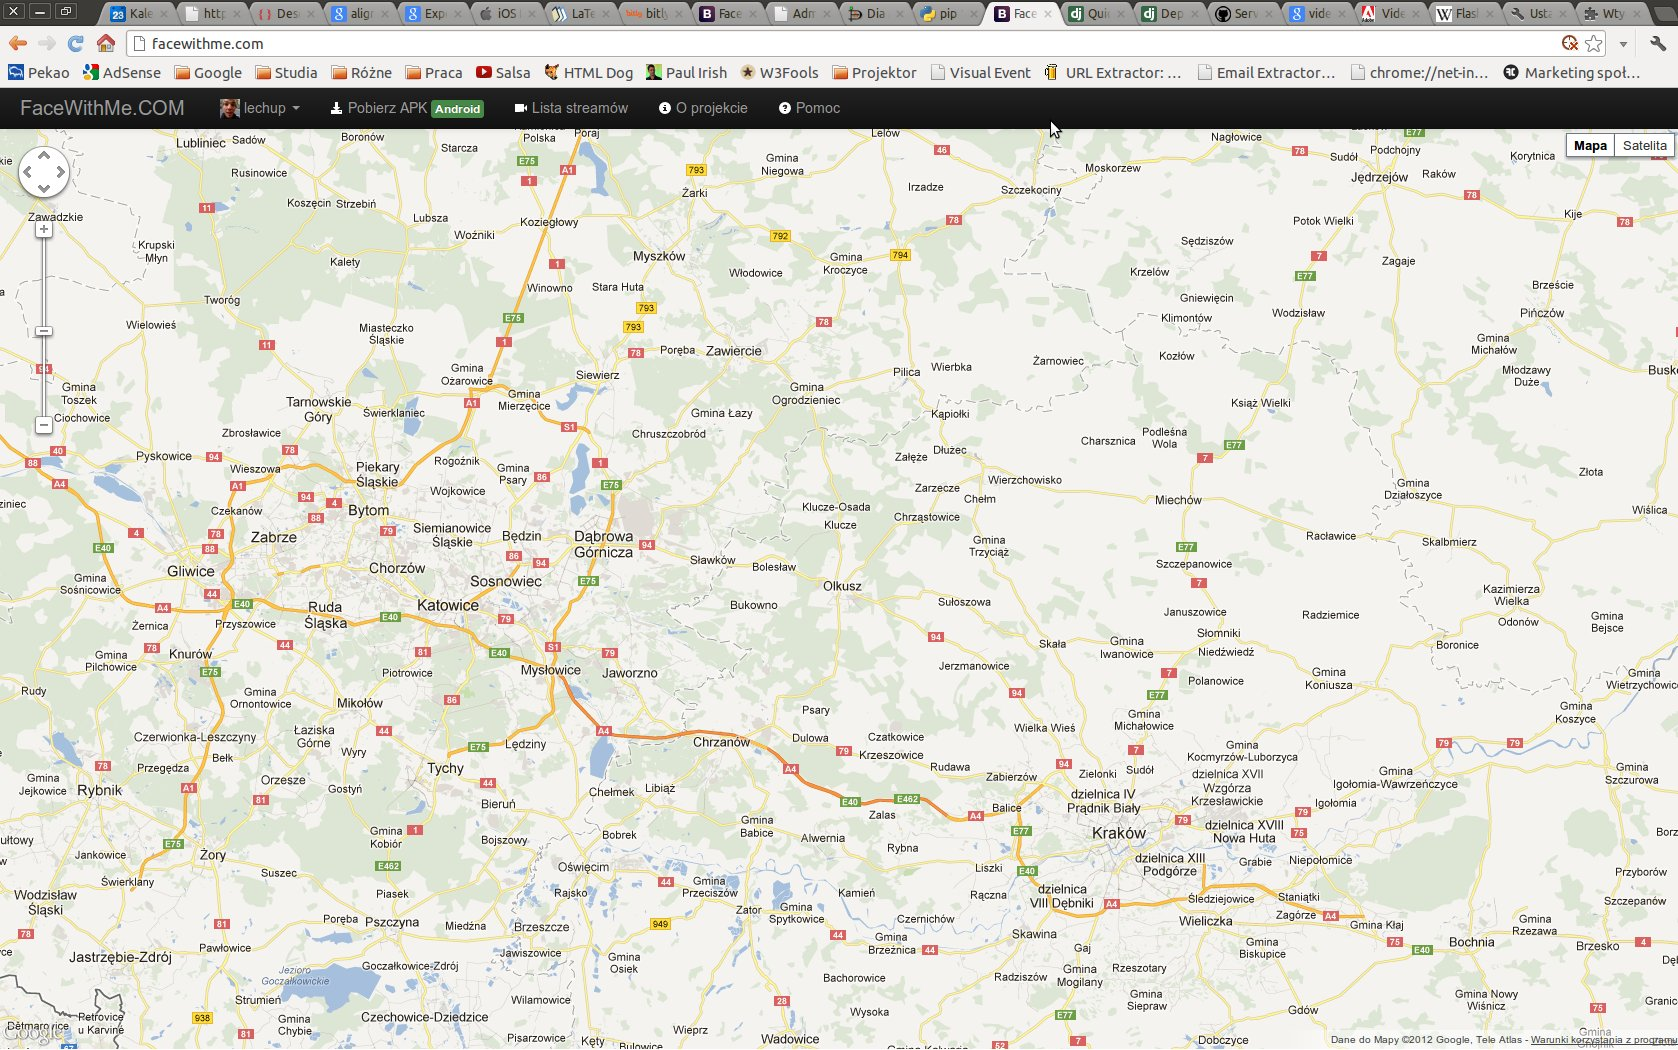
\includegraphics[width=\textwidth]{img/screens/interfejs_www/interaktywna-mapa.jpg}
        \end{center}
    }
    \item{funkcję automatycznej lokalizacji użytkownika i ustawienie pozycji mapy zgodnie z nią (\url{http://facewithme.com})}
    \item{listowanie wszystkich stream'ów nadawanych w systemie z podziałem na kategorie  (\url{http://facewithme.com/stream/list})
        \begin{center}
            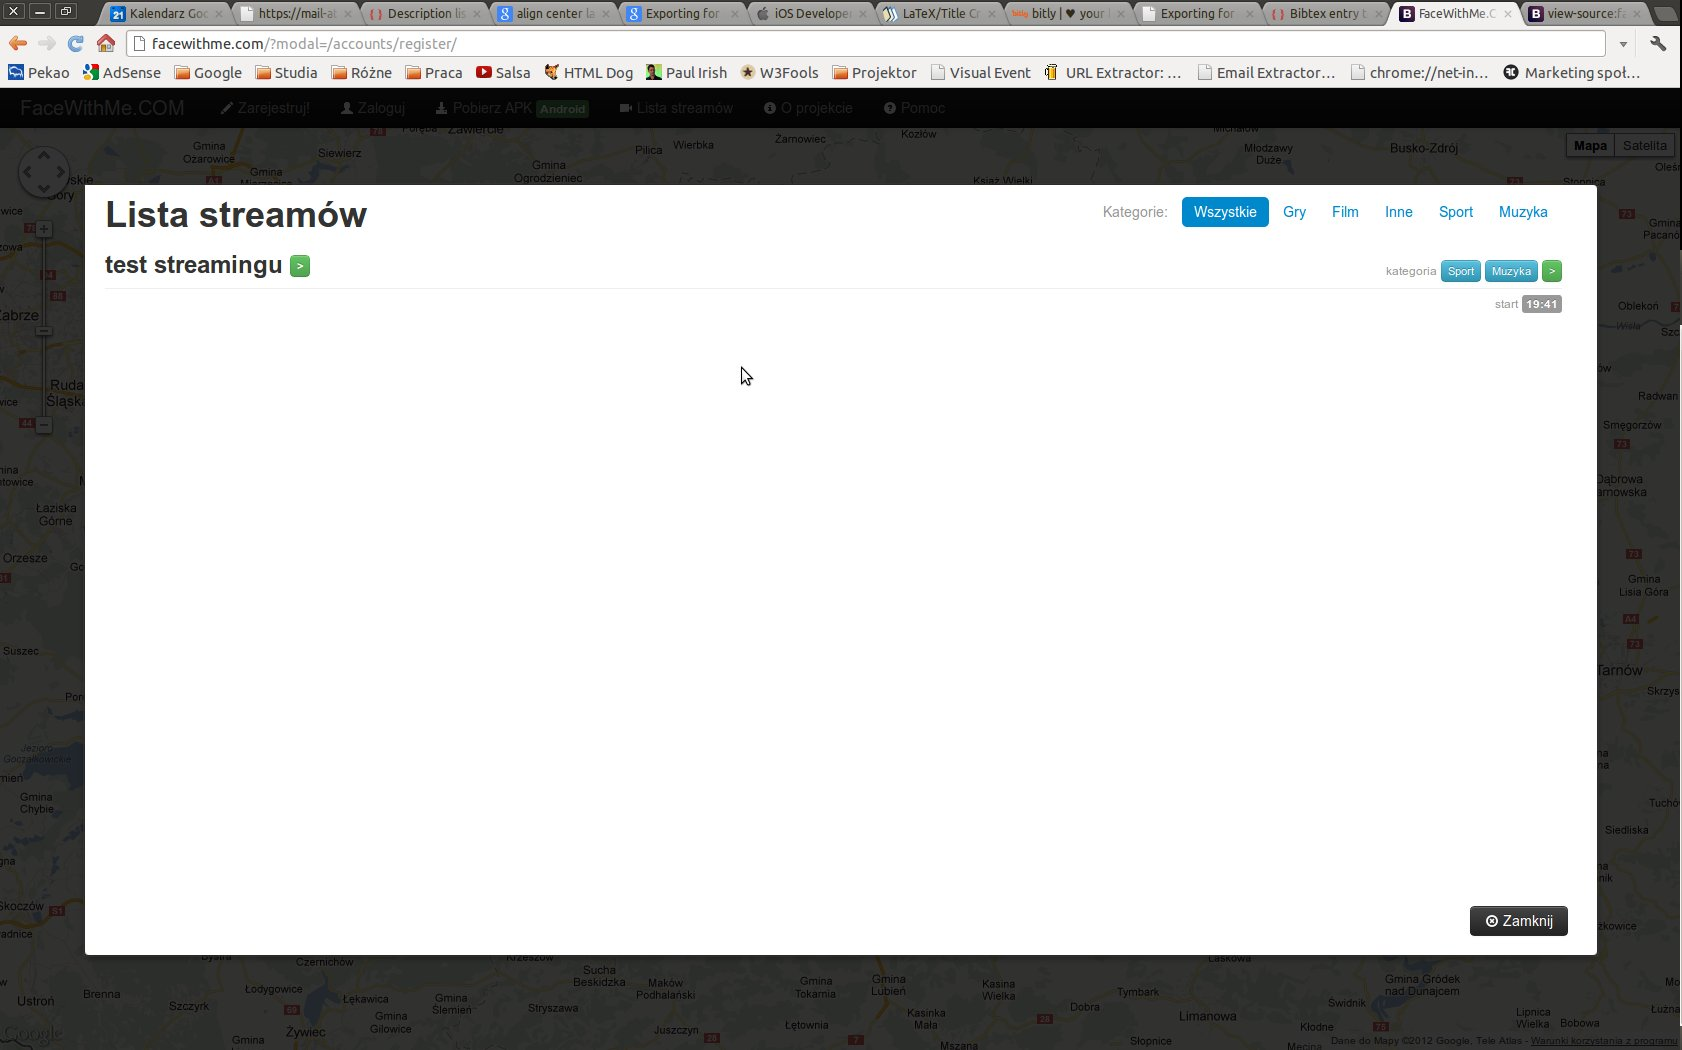
\includegraphics[width=\textwidth]{img/screens/interfejs_www/lista-streamow.jpg}
        \end{center}
    }
    \item{wyświetlanie Browser Receiver'a
        \begin{center}
            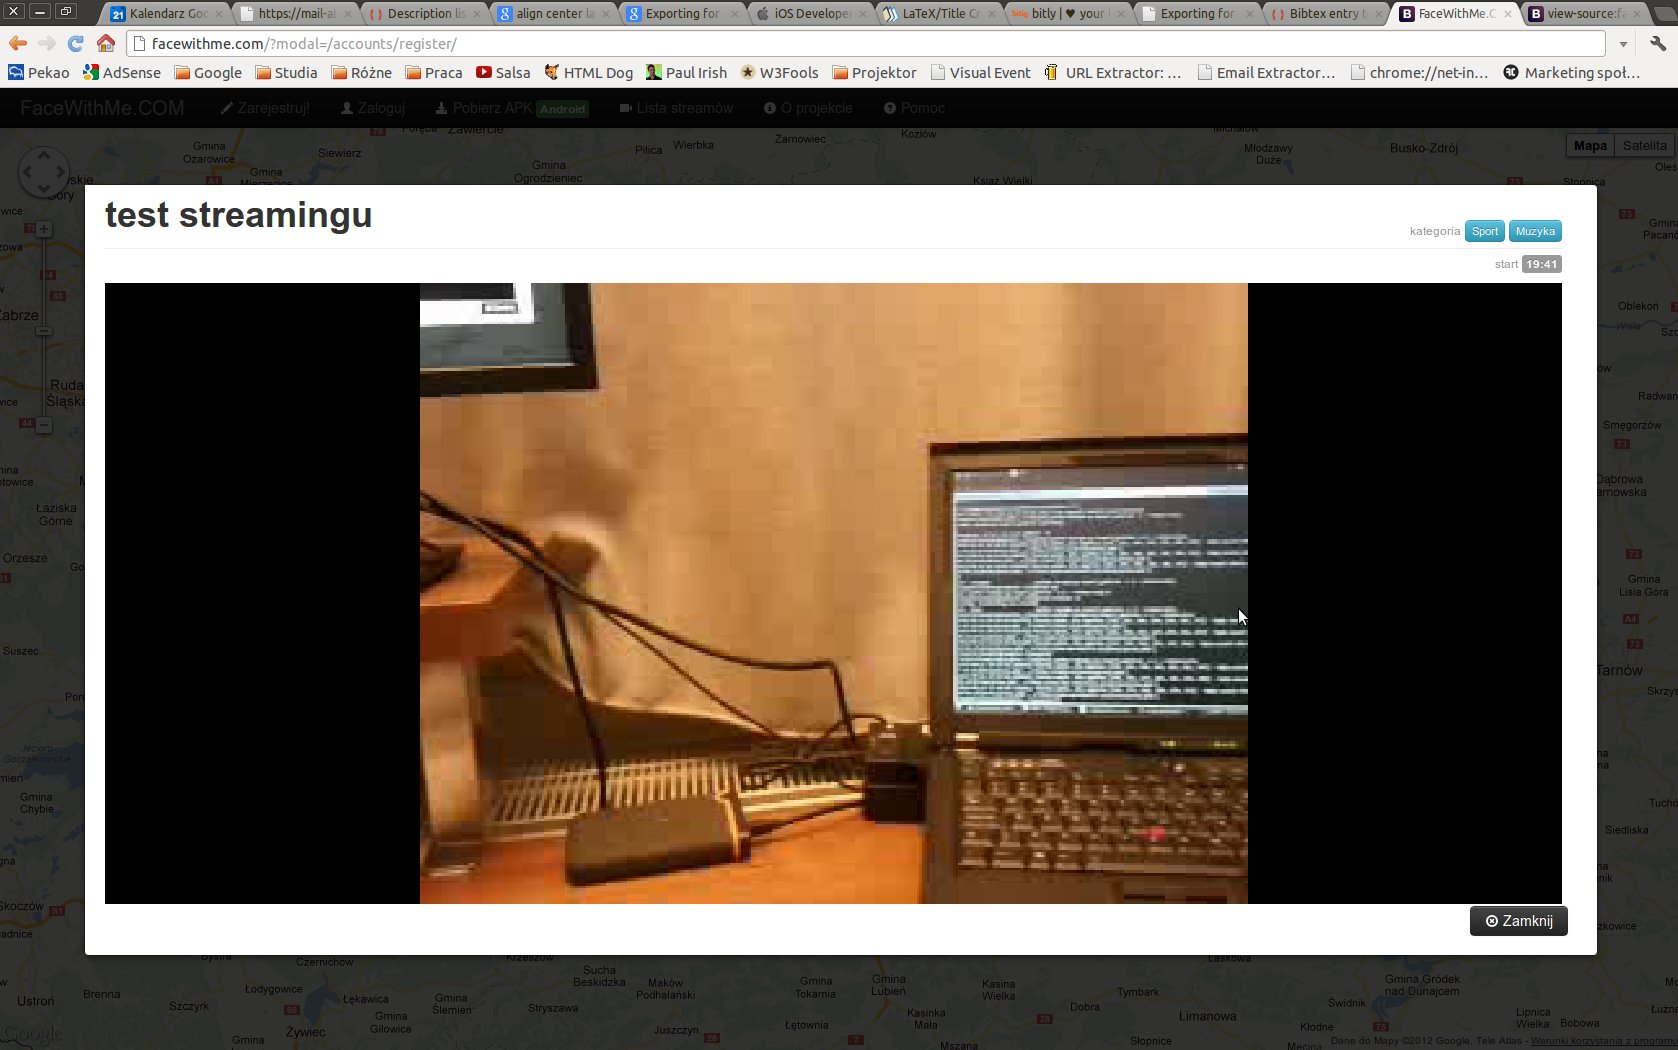
\includegraphics[width=\textwidth]{img/screens/interfejs_www/browser-receiver.jpg}
        \end{center}
    }
\end{packed_item}

\newpage
\textbf{Mobile Broadcaster}
\begin{packed_item}
    \item{panel udostępniania stream'u wideo}
    \item{stream'ing wideo}
    \item{ustawianie jakości stream'u w trakcie nadawania}
    \item{panel ustawień aplikacji}
    \item{panel DEBUG aplikacji}
\end{packed_item}

\begin{figure}[h]
        \centering
        \begin{subfigure}[b]{0.3\textwidth}
                \centering
                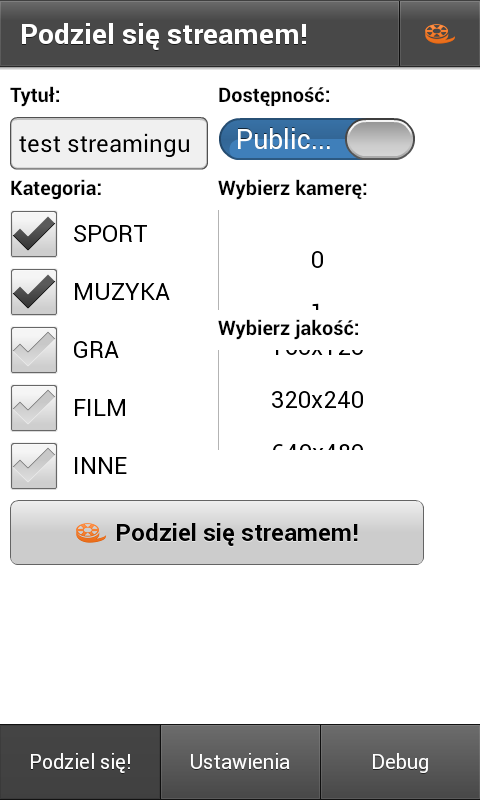
\includegraphics[width=\textwidth]{img/screens/mobile_broadcaster/panel-udostepniania-streamu.png}
                \caption{panel udostępniania stream'u}
        \end{subfigure}%
        ~ %add desired spacing between images, e. g. ~, \quad, \qquad etc. 
          %(or a blank line to force the subfigure onto a new line)
        \begin{subfigure}[b]{0.3\textwidth}
                \centering
                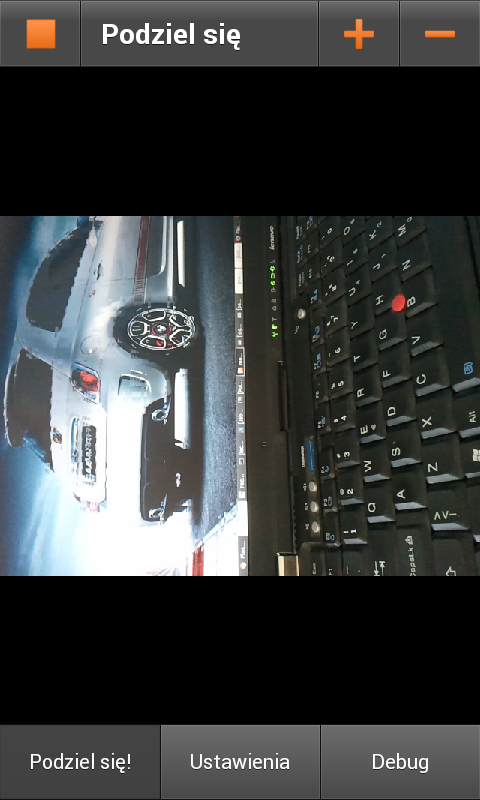
\includegraphics[width=\textwidth]{img/screens/mobile_broadcaster/streaming-wideo.png}
                \caption{stream'ing wideo}
        \end{subfigure}
        ~ %add desired spacing between images, e. g. ~, \quad, \qquad etc. 
          %(or a blank line to force the subfigure onto a new line)
        \begin{subfigure}[b]{0.3\textwidth}
                \centering
                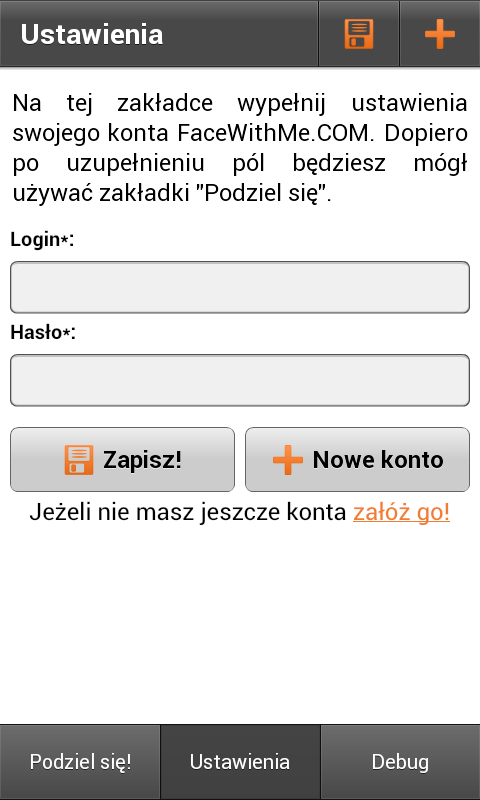
\includegraphics[width=\textwidth]{img/screens/mobile_broadcaster/panel-ustawien.png}
                \caption{panel ustawień aplikacji}
        \end{subfigure}
\end{figure}

\begin{figure}[h]
        \centering
        \begin{subfigure}[b]{0.3\textwidth}
                \centering
                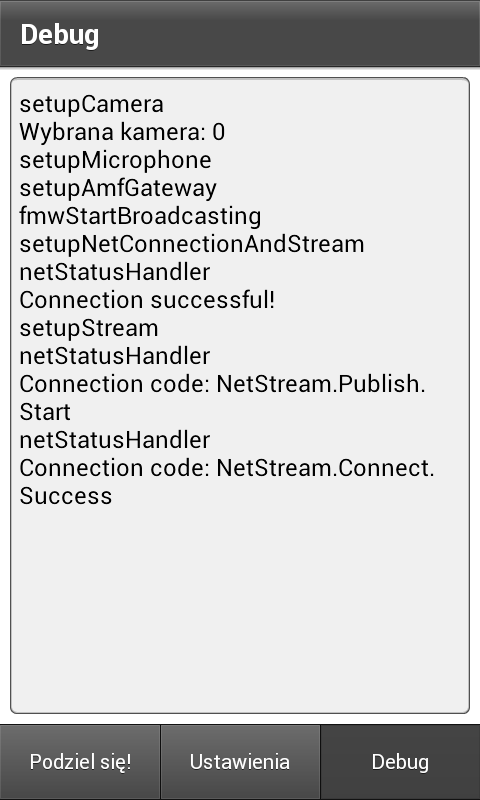
\includegraphics[width=\textwidth]{img/screens/mobile_broadcaster/panel-debug.png}
                \caption{panel DEBUG aplikacji}
        \end{subfigure}%
        ~ %add desired spacing between images, e. g. ~, \quad, \qquad etc. 
          %(or a blank line to force the subfigure onto a new line)
        \begin{subfigure}[b]{0.3\textwidth}
                \centering
                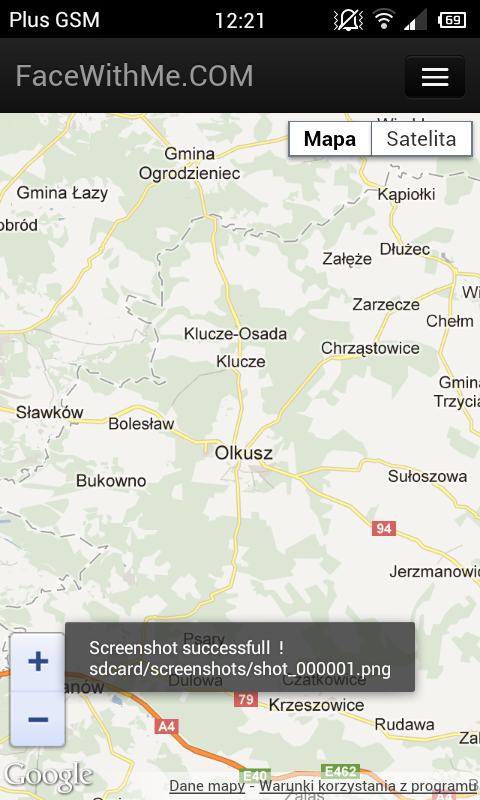
\includegraphics[width=\textwidth]{img/screens/mobile_broadcaster/interfejs-www.png}
                \caption{Interfejs WWW}
        \end{subfigure}
\end{figure}

\section{Co wymaga usprawnienia}

Przy implementacji prototypu systemu, nie skupiano się na sprawach pobocznych jak interfejs czy komunikacja z użytkownikiem. Głównie kierowano się intencją przetestowania w praktyce działania technologii Adobe P2P Multicast'ing. Dlatego też system wymaga znacznej ilości poprawek zanim może zacząć być wykorzystywany publicznie. Przygotowany prototyp traktować można jako bazę wyjściową do zapoznania się z działaniem i wydajnością technologii. Główne braki prototypu systemu to:

\begin{packed_item}
    \item{brak szyfrowania połączeń HTTP pomiędzy użytkownikiem a systemem, dotyczy także logowania}
    \item{brak jakiejkolwiek autoryzacji serwera RTMFP, jest dostępny publicznie}
    \item{brak zabezpieczenia publicznego/prywatnego streamu wideo}
    \item{brak całego Mobile Receiver'a}
    \item{brak całego Browser Broadcaster'a}
    \item{panel DEBUG w Mobile Broadcasterz'e}
    \item{brak obrotu komponentu kamery względem obrócenia urządzenia w Mobile Broadcasterz'e co skutkuje przesuwaniem obrazu kamery góra/dół, gdy kamera fizycznie poruszana jest prawo/lewo}
    \item{brak automatycznego usuwania stream'u z Interfejsu WWW w przypadku nieoczekiwanego przerwania działania Mobile Broadcaster'a}
    \item{brak komunikatów skierowanych do użytkownika Mobile Broadcaster'a, informujących o stanie lub błędach aplikacji}
    \item{brak wyłączania trybu czuwania urządzenia podczas udostępniania stream'u}
    \item{brak aplikacji na iOS -- Głównym powodem dla którego nie udało się stworzyć i przetestować aplikacji na platformę iOS jest koszt licencji Apple Developer Account (99\$), jaki trzeba ponieść, aby dostać możliwość umieszczania aplikacji na Apps Market oraz testowania aplikacji na własnym telefonie (szczegóły można znaleźć \cite{UnknAuth11}). Z powodu zastosowania technologii Adobe AIR for Mobile, nie ma możliwości testowania aplikacji za pomocą XCode i wirtualnego środowiska iOS. Z tego powodu dostępność komputerów Mac na uczelni na wiele się nie zdała. }
    \item{brak środowiska testującego oraz testów kodu źródłowego Adobe Flash Platform, zarówno kodu Adobe AIR for Mobile jak i Adobe Flash}
\end{packed_item}

\newpage
\section{Dokumentacja}
Zgodnie z filozofią metodyki,,XP'' (szczegóły \namedref{sec:ZMTOzalozenia}), dokumentacja projektu sprowadza się do opisu architektury oraz komentarzy kodu, testów oraz komentarzy do testów. Unika się tworzenia bazy wiedzy, która najczęściej jest po pewnym czasie nieaktualizowana.

Dlatego też, aby zapoznać się z działaniem systemu należy przejrzeć architekturę systemu, a następnie zapoznać się bezpośrednio z kodem źródłowym i zawartymi w nim komentarzami.

\subsection{Uruchomienie systemu}

Aby uruchomić system z kodu źródłowego należy:

\begin{packed_item}
    \item{\textbf{Interfejs WWW} -- Uruchomić aplikację Django, znajdującą się w dołączonym kodzie źródłowym w katalogu \texttt{./src/Django/facewithme/}. Wymagane do uruchomienia biblioteki Python'owskiego w formacie pliku wymagań programu PIP znajdują się w \texttt{./src/Django/facewithme/requirements/requirements.txt}. Instrukcja instalacji i wdrożenia aplikacji Django znajduje się tutaj: \url{https://docs.djangoproject.com/en/1.4/}. System wdrożony został przy wykorzystaniu Django 1.4.1}
    \item{\textbf{Serwer RTMFP} -- Uruchomić serwer  Cumulus. Instrukcja instalacji znajduje się na stronie \url{https://github.com/OpenRTMFP/Cumulus/wiki/Installation}. Dodatkowo należy umieścić serwer na liście dostępnych serwerów w panelu administracyjnym aplikacji Django. Domyślnie, dodawane stream'y losują jeden z dostępnych serwerów RTMFP. Można pokusić się o implementację algorytmu rozkładającego obciążenie bardziej równomiernie np. Round Robin.}
    \item{\textbf{Browser Receiver}, należy tak skonfigurować dołączanie obiektu flash, aby przekazywać informację na temat AMFGateway. Można do tego wykorzystać zmienną amfgateway dodając ją w widokach wyświetlających Browser Receiver. Domyślnie ustawiona jest na wartość \texttt{http://facewithme.com/amf/}.}
    \item{\textbf{Mobile Broadcaster}, należy uruchomić, zainstalować i skonfigurować środowisko Flash Develop zgodnie z tą instrukcją \url{http://www.flashdevelop.org/wikidocs/index.php?title=Configuration}. W plikach źródłowych odnaleźć domyślną konfigurację AMFGateway (\texttt{./src/Flex/FaceWithMe Mobile/src/Main.mxml}) i poprawić ją na adres skonfigurowanego wcześniej Interfejsu WWW. Skompilować projekt oraz stworzyć odpowiednie paczki instalacyjne dla platform docelowych (Android / iOS).}
\end{packed_item}

W razie problemów z wyświetlaniem się stream'u należy zapoznać się z plikiem pomocy \url{http://facewithme.com/help/}.

\subsection{Testy automatyczne}

Część Interfejsu WWW systemu posiada zalążki testów jednostkowych. Dotyczą one poprawnego wyświetlania widoków. Aby uruchomić testy, należy przejść do katalogu z z kodem źródłowym Django (\texttt{./src/Dajango/facewithme/}), a następnie uruchomić polecenie:

\lstset{language=Bash}
\begin{lstlisting}
python manage.py test core
\end{lstlisting}

O poprawnym wykonaniu testów informuje nas konsola, której wyjście zawiera:
\begin{lstlisting}
Creating test database for alias 'default'...
......
----------------------------------------------------------------------
Ran 6 tests in 0.822s

OK
Destroying test database for alias 'default'...
\end{lstlisting}

\subsection{Przeprowadzone testy}

System testowany był na kilku platformach. Poszczególne części systemu nie wykazywały błędnego zachowania:

\begin{packed_item}
    \item{Interfejs WWW z Browser Receiver -- Google Chrome (21.0.1180.89) + Flash Player (11.3.31.232)/Linux; FireFox 15.0.1 + Flash Player 11.2.202.238/Linux; Google Google Chrome (21.0.1180.89) + Flash Player (11.3.31.232)/Windows 7;  FireFox 15 + Flash Player 11.2.202.238/Windows 7}
    \item{Mobile Broadcaster -- Adobe AIR 3.4.0.254/Android 4.04/Samsung Galaxy S I, Adobe AIR 3.4.0.254/Android 3.2/Samsung Galaxy Tab 10.1}
\end{packed_item}

\subsection{Bezpieczeństwo}

Bardzo ważnym aspektem docelowego systemu powinno być bezpieczeństwo. Niżej wyszczególniono elementy prototypu systemu, które mają bezpośredni związek z bezpieczeństwem i sugerowane poprawki, które pomogą zabezpieczyć system.

\begin{packed_item}
    \item{Dzięki zastosowaniu technologii Adobe Flash Platform oraz wykorzystaniu protokołu RTMFP, transmisja danych pomiędzy Mobile Broadcaster'em oraz Browser Receiver'em jest szyfrowana. Szyfrowanie odbywa się za pomocą 128-bitowego klucza. Szczegółowe informacje można uzyskać pod tym adresem \url{http://help.adobe.com/en_US/flashmediaserver/techoverview/WS5b3ccc516d4fbf351e63e3d119ed944af6-7ffb.html}}
    \item{Komunikacja pomiędzy Interfejsem WWW, a Browser Receiver'em oraz Mobile Receiver'em, odbywająca się za pomocą AMFGateway powinna odbywać się za pomocą protokołu HTTPS, nie HTTP jak w prototypie.}
    \item{Logowanie do panelu administracyjnego oraz logowanie użytkowników powinno wykorzystywać protokół HTTPS, nie HTTP jak w prototypie.}
    \item{Sugeruje się przejście na HTTPS w każdej komunikacji nawiązywanej pomiędzy użytkownikiem, a Interfejsem WWW, nie HTTP jak w prototypie.}
    \item{Serwer RTMFP (Cumulus), nie udostępnia żadnego sposobu na autoryzację połączeń. Najprostszym sposobem na ograniczenie wykorzystania przez nieautoryzowanych użytkowników jest sprawdzanie \texttt{swfUrl} połączającego się klienta za pomocą rozszerzenia serwera wykorzystującego zdarzenie \texttt{onConnection} (szczegóły w dokumentacji Cumulus \url{https://github.com/OpenRTMFP/Cumulus/wiki/Server-Application,-API})}
\end{packed_item}

\newpage
\section{Wydajność P2P Multicast'ing w Adobe Flash Platform}

W tym rozdziale chciano poruszyć temat związany z wydajnością transmisji wideo za pomocą technologii P2P Multicast'ing. Kryterium jakie chcemy sprawdzać to opóźnienie transmisji wideo względem obrazu oryginalnego oraz jego płynność. Opóźnienie jest wyrażone w sekundach. Płynność określono jako jedną z możliwości:
\begin{packed_item}
    \item{obraz całkowicie płynny -- obraz zachowuje płynność ciągle}
    \item{obraz płynny -- obraz od czasu do czasu wstrzymuje się, większą część czasu jest płynny}
    \item{obraz skaczący -- obraz nie jest płynny, posiada natomiast więcej niż jedną klatkę na sekundę}
    \item{obraz poklatkowy -- obraz nie jest całkowicie płynny, posiada mniej niż jedną klatkę na sekundę}
    \item{obraz nieczytelny -- obraz pojawia się we fragmentach, wyświetlają się pomniejsze}
\end{packed_item}

Środowisko testowe składa się z dwóch komputerów klientów, na których uruchomiono przeglądarkę Google Chrome i włączono Browser Receiver dla stream'u udostępnianego przez Mobile Broadcaster uruchomionego na Adobe AIR 3.4.0.254/Android 3.2/Samsung Galaxy Tab 10.1. Aplikacja mobilna wysyłanie stream'u wideo przeprowadza za pomocą łącza ADSL (połączenie WiFi przez router) o parametrach faktycznych 8 Mb/s pobieranie, 1 Mb/s wysyłanie danych. Alternatywnym połączeniem Mobile Broadcaster'a jest darmowy internet od Aero2 w technologii HSPA/HSPA+ o parametrach faktycznych 0.5 Mb/s pobieranie, 0.4 Mb/s wysyłanie danych. Komputery klienckie są połączone do tej samej sieci LAN, korzystającej z wcześniej wymienionego łącza ADSL. Test prędkości łącz został wykonany za pomocą serwisu \url{http://speedtest.net}.

Wpływ na badane kryteria mają parametry:
\begin{packed_item}
    \item{Rozdzielczość obrazu w transmisji wideo, która jest przekazywana.}
    \item{Ilość klientów uczestniczących w transmisji P2P Multicast.}
\end{packed_item}

Tabela przedstawiająca płynność transmisji oglądanej na ekranie Browser Receiver'a, względem rozdzielczości przesyłanego strumienia w pikselach. Dla dwóch włączonych Browser Reveiver'ów, po jednej instancji per komputer klient:
\begin{table}[h]
    \centering
    \begin{tabular}{|l|l|l|l|l|}
        \hline
        & 80x60px & 160x120px & 320x240px & 640x480px \\
        \hline
        ADSL
        &
        obraz całkowicie płynny 
        &
        obraz całkowicie płynny
        &
        obraz płynny
        &
        obraz skaczący
        \\
        \hline
        Aero2
        &
        obraz płynny
        &
        obraz poklatkowy
        &
        obraz nieczytelny
        &
        obraz nieczytelny
        \\
        \hline
    \end{tabular}
\end{table}

Tabela przedstawiająca opóźnienie transmisji oglądanej na ekranie Browser Receiver'a, względem rozdzielczości przesyłanego strumienia w pikselach. Dla dwóch włączonych Browser Reveiver'ów, po jednej instancji per komputer klient:
\begin{table}[h]
    \centering
    \begin{tabular}{|l|l|l|l|l|}
        \hline
        & 80x60px & 160x120px & 320x240px & 640x480px \\
        \hline
        ADSL
        &
        opóźnienie 0s
        &
        opóźnienie 0s
        &
        opóźnienie 0,1s
        &
        opóźnienie 0-1s \\
        \hline
        Aero2
        &
        opóźnienie 0,1-0,5s
        &
        opóźnienie 2-3s
        &
        opóźnienie 4-5s
        &
        opóźnienie ~40s \\
        \hline
    \end{tabular}
\end{table}

\newpage
Tabela przedstawiająca płynność transmisji oglądanej na ekranie Browser Receiver'a, względem rozdzielczości przesyłanego strumienia w pikselach. Dla sześciu włączonych Browser Reveiver'ów, po trzy instancje per komputer klient:
\begin{table}[h]
    \centering
    \begin{tabular}{|l|l|l|l|l|}
        \hline
        & 80x60px & 160x120px & 320x240px & 640x480px \\
        \hline
        ADSL
        &
        obraz całkowicie płynny 
        &
        obraz płynny
        &
        obraz płynny
        &
        obraz poklatkowy
        \\
        \hline
        Aero2
        &
        obraz płynny
        &
        obraz poklatkowy
        &
        obraz poklatkowy
        &
        obraz nieczytelny
        \\
        \hline
    \end{tabular}
\end{table}

Tabela przedstawiająca opóźnienie transmisji oglądanej na ekranie Browser Receiver'a, względem rozdzielczości przesyłanego strumienia w pikselach. Dla sześciu włączonych Browser Reveiver'ów, po trzy instancje per komputer klient:
\begin{table}[h]
    \centering
    \begin{tabular}{|l|l|l|l|l|}
        \hline
        & 80x60px & 160x120px & 320x240px & 640x480px \\
        \hline
        ADSL
        &
        opóźnienie 0s
        &
        opóźnienie 0-0,3s
        &
        opóźnienie 0-0,5s
        &
        opóźnienie 0,5-2s \\
        \hline
        Aero2
        &
        opóźnienie 0-3s
        &
        opóźnienie 30s
        &
        opóźnienie 35s
        &
        opóźnienie 45s \\
        \hline
    \end{tabular}
\end{table}

\newpage
\section{Wnioski}

W tym rozdziale zaprezentowane są wnioski powstałe podczas implementacji prototypu systemu.

\begin{packed_item}
    \item{Im gorsze połączenie Mobile Broadcast'era tym gorsza możliwa jakość przesyłu wideo.}
    \item{Im gorsze połączenie Mobile Broadcast'era, a ilość Browser Reveicer'ów większa tym lepsza płynność transmisji wideo.}
    \item{Im lepsze połączenie Mobile Broadcast'era tym lepsza możliwa jakość przesyłu wideo.}
    \item{Im więcej klientów Browser Reveiver'a podłączone do stream'u tym większe możliwe opóźnienie.}
    \item{Aby stworzyć aplikację na iOS za pomocą Adobe AIR for Mobile należy posiadać Apple Developer Account.}
    \item{Adobe P2P Multicast'ing działa i wydaje się sensowną technologią do wdrożenia projektowanego systemu.}
    \item{Aby publicznie udostępnić system należy sporo rzeczy poprawić, w szczególności popracować nad bezpieczeństwem systemu.}
    \item{Wszystkie wykorzystane przy implementacji prototypu technologie spełniają swoją powierzoną rolę.}
    \item{Istnieje ryzyko stworzenia systemu służącego do permanentnej inwigilacji...}
    \item{Metodyka ,,XP'' ma duże szanse powodzenia przy prowadzeniu szybko zmieniającego się projektu przy udziale niedużej grupy projektowej.}
    \item{Przygotowywanie ekranów do kart wymagań za pomocą programu graficznego jest pracochłonną czynnością, dużo lepiej powinny sprawdzić odręczne szkice i ,,cyfryzacja'' za pomocą zdjęć np. telefonem komórkowym.}
\end{packed_item}

\newpage
%---------------------------------------------------------------------------
